% GNUPLOT: LaTeX picture with Postscript
\begingroup
  \makeatletter
  \providecommand\color[2][]{%
    \GenericError{(gnuplot) \space\space\space\@spaces}{%
      Package color not loaded in conjunction with
      terminal option `colourtext'%
    }{See the gnuplot documentation for explanation.%
    }{Either use 'blacktext' in gnuplot or load the package
      color.sty in LaTeX.}%
    \renewcommand\color[2][]{}%
  }%
  \providecommand\includegraphics[2][]{%
    \GenericError{(gnuplot) \space\space\space\@spaces}{%
      Package graphicx or graphics not loaded%
    }{See the gnuplot documentation for explanation.%
    }{The gnuplot epslatex terminal needs graphicx.sty or graphics.sty.}%
    \renewcommand\includegraphics[2][]{}%
  }%
  \providecommand\rotatebox[2]{#2}%
  \@ifundefined{ifGPcolor}{%
    \newif\ifGPcolor
    \GPcolortrue
  }{}%
  \@ifundefined{ifGPblacktext}{%
    \newif\ifGPblacktext
    \GPblacktextfalse
  }{}%
  % define a \g@addto@macro without @ in the name:
  \let\gplgaddtomacro\g@addto@macro
  % define empty templates for all commands taking text:
  \gdef\gplbacktext{}%
  \gdef\gplfronttext{}%
  \makeatother
  \ifGPblacktext
    % no textcolor at all
    \def\colorrgb#1{}%
    \def\colorgray#1{}%
  \else
    % gray or color?
    \ifGPcolor
      \def\colorrgb#1{\color[rgb]{#1}}%
      \def\colorgray#1{\color[gray]{#1}}%
      \expandafter\def\csname LTw\endcsname{\color{white}}%
      \expandafter\def\csname LTb\endcsname{\color{black}}%
      \expandafter\def\csname LTa\endcsname{\color{black}}%
      \expandafter\def\csname LT0\endcsname{\color[rgb]{1,0,0}}%
      \expandafter\def\csname LT1\endcsname{\color[rgb]{0,1,0}}%
      \expandafter\def\csname LT2\endcsname{\color[rgb]{0,0,1}}%
      \expandafter\def\csname LT3\endcsname{\color[rgb]{1,0,1}}%
      \expandafter\def\csname LT4\endcsname{\color[rgb]{0,1,1}}%
      \expandafter\def\csname LT5\endcsname{\color[rgb]{1,1,0}}%
      \expandafter\def\csname LT6\endcsname{\color[rgb]{0,0,0}}%
      \expandafter\def\csname LT7\endcsname{\color[rgb]{1,0.3,0}}%
      \expandafter\def\csname LT8\endcsname{\color[rgb]{0.5,0.5,0.5}}%
    \else
      % gray
      \def\colorrgb#1{\color{black}}%
      \def\colorgray#1{\color[gray]{#1}}%
      \expandafter\def\csname LTw\endcsname{\color{white}}%
      \expandafter\def\csname LTb\endcsname{\color{black}}%
      \expandafter\def\csname LTa\endcsname{\color{black}}%
      \expandafter\def\csname LT0\endcsname{\color{black}}%
      \expandafter\def\csname LT1\endcsname{\color{black}}%
      \expandafter\def\csname LT2\endcsname{\color{black}}%
      \expandafter\def\csname LT3\endcsname{\color{black}}%
      \expandafter\def\csname LT4\endcsname{\color{black}}%
      \expandafter\def\csname LT5\endcsname{\color{black}}%
      \expandafter\def\csname LT6\endcsname{\color{black}}%
      \expandafter\def\csname LT7\endcsname{\color{black}}%
      \expandafter\def\csname LT8\endcsname{\color{black}}%
    \fi
  \fi
    \setlength{\unitlength}{0.0500bp}%
    \ifx\gptboxheight\undefined%
      \newlength{\gptboxheight}%
      \newlength{\gptboxwidth}%
      \newsavebox{\gptboxtext}%
    \fi%
    \setlength{\fboxrule}{0.5pt}%
    \setlength{\fboxsep}{1pt}%
\begin{picture}(7360.00,10200.00)%
    \gplgaddtomacro\gplbacktext{%
      \csname LTb\endcsname%%
      \put(441,7172){\makebox(0,0)[r]{\strut{}$0$}}%
      \csname LTb\endcsname%%
      \put(441,7912){\makebox(0,0)[r]{\strut{}$1$}}%
      \csname LTb\endcsname%%
      \put(441,8653){\makebox(0,0)[r]{\strut{}$2$}}%
      \csname LTb\endcsname%%
      \put(441,9393){\makebox(0,0)[r]{\strut{}$3$}}%
      \csname LTb\endcsname%%
      \put(543,6986){\makebox(0,0){\strut{}$0$}}%
      \csname LTb\endcsname%%
      \put(1251,6986){\makebox(0,0){\strut{}$20$}}%
      \csname LTb\endcsname%%
      \put(1958,6986){\makebox(0,0){\strut{}$40$}}%
      \csname LTb\endcsname%%
      \put(2666,6986){\makebox(0,0){\strut{}$60$}}%
      \csname LTb\endcsname%%
      \put(3373,6986){\makebox(0,0){\strut{}$80$}}%
    }%
    \gplgaddtomacro\gplfronttext{%
      \csname LTb\endcsname%%
      \put(153,8282){\rotatebox{-270}{\makebox(0,0){\strut{}uptake / (mol/mol)}}}%
      \csname LTb\endcsname%%
      \put(1958,10064){\makebox(0,0){\strut{}\ce{CO2} / \ce{O2} (OFAST)}}%
      \colorrgb{0.58,0.00,0.83}%%
      \put(1312,9754){\makebox(0,0)[r]{\strut{}\footnotesize $y_\smallce{CO2} = 0.1$}}%
      \colorrgb{0.00,0.62,0.45}%%
      \put(2332,9754){\makebox(0,0)[r]{\strut{}\footnotesize $y_\smallce{CO2} = 0.5$}}%
      \colorrgb{0.00,0.45,0.70}%%
      \put(3352,9754){\makebox(0,0)[r]{\strut{}\footnotesize $y_\smallce{CO2} = 0.9$}}%
    }%
    \gplgaddtomacro\gplbacktext{%
      \csname LTb\endcsname%%
      \put(3935,7172){\makebox(0,0)[r]{\strut{}$0$}}%
      \csname LTb\endcsname%%
      \put(3935,7912){\makebox(0,0)[r]{\strut{}$1$}}%
      \csname LTb\endcsname%%
      \put(3935,8653){\makebox(0,0)[r]{\strut{}$2$}}%
      \csname LTb\endcsname%%
      \put(3935,9393){\makebox(0,0)[r]{\strut{}$3$}}%
      \csname LTb\endcsname%%
      \put(4037,6986){\makebox(0,0){\strut{}$0$}}%
      \csname LTb\endcsname%%
      \put(4791,6986){\makebox(0,0){\strut{}$20$}}%
      \csname LTb\endcsname%%
      \put(5545,6986){\makebox(0,0){\strut{}$40$}}%
      \csname LTb\endcsname%%
      \put(6299,6986){\makebox(0,0){\strut{}$60$}}%
      \csname LTb\endcsname%%
      \put(7053,6986){\makebox(0,0){\strut{}$80$}}%
    }%
    \gplgaddtomacro\gplfronttext{%
      \csname LTb\endcsname%%
      \put(5545,10064){\makebox(0,0){\strut{}\ce{CO2} / \ce{O2} (IAST)}}%
      \colorrgb{0.00,0.00,0.00}%%
      \put(5063,9754){\makebox(0,0)[r]{\strut{}$n_\smallce{CO2}$}}%
      \colorrgb{0.00,0.00,0.00}%%
      \put(5885,9754){\makebox(0,0)[r]{\strut{}$n_\smallce{O2}$}}%
    }%
    \gplgaddtomacro\gplbacktext{%
      \csname LTb\endcsname%%
      \put(441,3772){\makebox(0,0)[r]{\strut{}$0$}}%
      \csname LTb\endcsname%%
      \put(441,4512){\makebox(0,0)[r]{\strut{}$1$}}%
      \csname LTb\endcsname%%
      \put(441,5253){\makebox(0,0)[r]{\strut{}$2$}}%
      \csname LTb\endcsname%%
      \put(441,5993){\makebox(0,0)[r]{\strut{}$3$}}%
      \csname LTb\endcsname%%
      \put(543,3586){\makebox(0,0){\strut{}$0$}}%
      \csname LTb\endcsname%%
      \put(1251,3586){\makebox(0,0){\strut{}$20$}}%
      \csname LTb\endcsname%%
      \put(1958,3586){\makebox(0,0){\strut{}$40$}}%
      \csname LTb\endcsname%%
      \put(2666,3586){\makebox(0,0){\strut{}$60$}}%
      \csname LTb\endcsname%%
      \put(3373,3586){\makebox(0,0){\strut{}$80$}}%
    }%
    \gplgaddtomacro\gplfronttext{%
      \csname LTb\endcsname%%
      \put(153,4882){\rotatebox{-270}{\makebox(0,0){\strut{}uptake / (mol/mol)}}}%
      \csname LTb\endcsname%%
      \put(1958,6664){\makebox(0,0){\strut{}\ce{CH4} / \ce{O2} (OFAST)}}%
      \colorrgb{0.58,0.00,0.83}%%
      \put(1312,6354){\makebox(0,0)[r]{\strut{}\footnotesize $y_\smallce{CH4} = 0.1$}}%
      \colorrgb{0.00,0.62,0.45}%%
      \put(2332,6354){\makebox(0,0)[r]{\strut{}\footnotesize $y_\smallce{CH4} = 0.5$}}%
      \colorrgb{0.00,0.45,0.70}%%
      \put(3352,6354){\makebox(0,0)[r]{\strut{}\footnotesize $y_\smallce{CH4} = 0.9$}}%
    }%
    \gplgaddtomacro\gplbacktext{%
      \csname LTb\endcsname%%
      \put(3935,3772){\makebox(0,0)[r]{\strut{}$0$}}%
      \csname LTb\endcsname%%
      \put(3935,4512){\makebox(0,0)[r]{\strut{}$1$}}%
      \csname LTb\endcsname%%
      \put(3935,5253){\makebox(0,0)[r]{\strut{}$2$}}%
      \csname LTb\endcsname%%
      \put(3935,5993){\makebox(0,0)[r]{\strut{}$3$}}%
      \csname LTb\endcsname%%
      \put(4037,3586){\makebox(0,0){\strut{}$0$}}%
      \csname LTb\endcsname%%
      \put(4791,3586){\makebox(0,0){\strut{}$20$}}%
      \csname LTb\endcsname%%
      \put(5545,3586){\makebox(0,0){\strut{}$40$}}%
      \csname LTb\endcsname%%
      \put(6299,3586){\makebox(0,0){\strut{}$60$}}%
      \csname LTb\endcsname%%
      \put(7053,3586){\makebox(0,0){\strut{}$80$}}%
    }%
    \gplgaddtomacro\gplfronttext{%
      \csname LTb\endcsname%%
      \put(5545,6664){\makebox(0,0){\strut{}\ce{CH4} / \ce{O2} (IAST)}}%
      \colorrgb{0.00,0.00,0.00}%%
      \put(5063,6354){\makebox(0,0)[r]{\strut{}$n_\smallce{CH4}$}}%
      \colorrgb{0.00,0.00,0.00}%%
      \put(5885,6354){\makebox(0,0)[r]{\strut{}$n_\smallce{O2}$}}%
    }%
    \gplgaddtomacro\gplbacktext{%
      \csname LTb\endcsname%%
      \put(441,595){\makebox(0,0)[r]{\strut{}$0$}}%
      \csname LTb\endcsname%%
      \put(441,1261){\makebox(0,0)[r]{\strut{}$1$}}%
      \csname LTb\endcsname%%
      \put(441,1928){\makebox(0,0)[r]{\strut{}$2$}}%
      \csname LTb\endcsname%%
      \put(441,2594){\makebox(0,0)[r]{\strut{}$3$}}%
      \csname LTb\endcsname%%
      \put(543,409){\makebox(0,0){\strut{}$0$}}%
      \csname LTb\endcsname%%
      \put(1251,409){\makebox(0,0){\strut{}$20$}}%
      \csname LTb\endcsname%%
      \put(1958,409){\makebox(0,0){\strut{}$40$}}%
      \csname LTb\endcsname%%
      \put(2666,409){\makebox(0,0){\strut{}$60$}}%
      \csname LTb\endcsname%%
      \put(3373,409){\makebox(0,0){\strut{}$80$}}%
    }%
    \gplgaddtomacro\gplfronttext{%
      \csname LTb\endcsname%%
      \put(153,1594){\rotatebox{-270}{\makebox(0,0){\strut{}uptake / (mol/mol)}}}%
      \csname LTb\endcsname%%
      \put(1958,130){\makebox(0,0){\strut{}pressure / atm}}%
      \csname LTb\endcsname%%
      \put(1958,3264){\makebox(0,0){\strut{}\ce{CH4} / \ce{CO2} (OFAST)}}%
      \colorrgb{0.58,0.00,0.83}%%
      \put(1312,2954){\makebox(0,0)[r]{\strut{}\footnotesize $y_\smallce{CH4} = 0.1$}}%
      \colorrgb{0.00,0.62,0.45}%%
      \put(2332,2954){\makebox(0,0)[r]{\strut{}\footnotesize $y_\smallce{CH4} = 0.5$}}%
      \colorrgb{0.00,0.45,0.70}%%
      \put(3352,2954){\makebox(0,0)[r]{\strut{}\footnotesize $y_\smallce{CH4} = 0.9$}}%
    }%
    \gplgaddtomacro\gplbacktext{%
      \csname LTb\endcsname%%
      \put(3935,595){\makebox(0,0)[r]{\strut{}$0$}}%
      \csname LTb\endcsname%%
      \put(3935,1261){\makebox(0,0)[r]{\strut{}$1$}}%
      \csname LTb\endcsname%%
      \put(3935,1928){\makebox(0,0)[r]{\strut{}$2$}}%
      \csname LTb\endcsname%%
      \put(3935,2594){\makebox(0,0)[r]{\strut{}$3$}}%
      \csname LTb\endcsname%%
      \put(4037,409){\makebox(0,0){\strut{}$0$}}%
      \csname LTb\endcsname%%
      \put(4791,409){\makebox(0,0){\strut{}$20$}}%
      \csname LTb\endcsname%%
      \put(5545,409){\makebox(0,0){\strut{}$40$}}%
      \csname LTb\endcsname%%
      \put(6299,409){\makebox(0,0){\strut{}$60$}}%
      \csname LTb\endcsname%%
      \put(7053,409){\makebox(0,0){\strut{}$80$}}%
    }%
    \gplgaddtomacro\gplfronttext{%
      \csname LTb\endcsname%%
      \put(5545,130){\makebox(0,0){\strut{}pressure / atm}}%
      \csname LTb\endcsname%%
      \put(5545,3264){\makebox(0,0){\strut{}\ce{CH4} / \ce{CO2} (IAST)}}%
      \colorrgb{0.00,0.00,0.00}%%
      \put(5063,2954){\makebox(0,0)[r]{\strut{}$n_\smallce{CH4}$}}%
      \colorrgb{0.00,0.00,0.00}%%
      \put(5885,2954){\makebox(0,0)[r]{\strut{}$n_\smallce{CO2}$}}%
    }%
    \gplbacktext
    \put(0,0){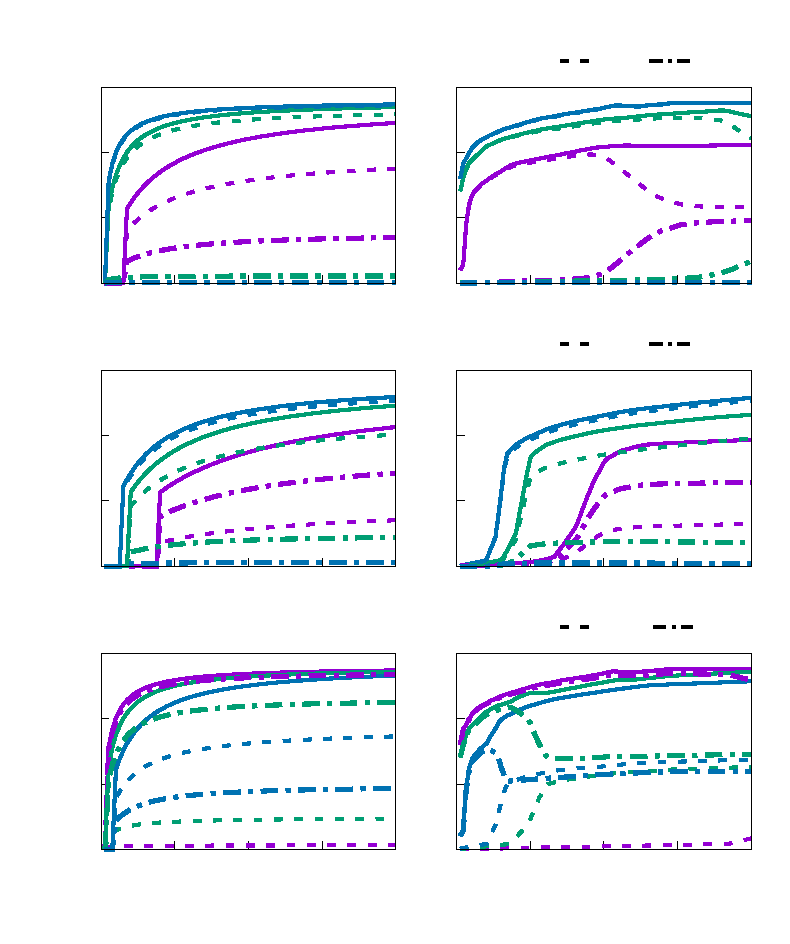
\includegraphics{cu-dhbc-loadings}}%
    \gplfronttext
  \end{picture}%
\endgroup
